\documentclass[a4paper,12pt,openany]{book}
\usepackage [utf8]{inputenc}
\usepackage [french]{babel}
\usepackage [T1]{fontenc}
\usepackage{listings}
\usepackage{graphicx}
\usepackage{verbatim}

%%configuration de listings
\lstset{
language=c,
basicstyle=\ttfamily\small, 
identifierstyle=\color{red}, 
keywordstyle=\color{blue}, 
stringstyle=\color{black!60}, 
commentstyle=\it\color{green!95!yellow!1}, 
columns=flexible, 
tabsize=1, 
extendedchars=true, 
showspaces=false, 
showstringspaces=false, 
numbers=left, 
numberstyle=\tiny, 
breaklines=true, 
breakautoindent=true, 
captionpos=b
}

%coloration syntaxique
\usepackage{xcolor}
\definecolor{Zgris}{rgb}{0.87,0.85,0.85}

\newsavebox{\BBbox}
\newenvironment{DDbox}[1]{
\begin{lrbox}{\BBbox}\begin{minipage}{\linewidth}}
{\end{minipage}\end{lrbox}\noindent\colorbox{Zgris}{\\usebox{\BBbox}}
[.5cm]}

%Pour l espace entre la section et la chapitre (qui est trop grand).
\usepackage{titlesec}

\titleformat{\chapter}[block]
  {\normalfont\Huge\bfseries}% font of number
  {\chaptertitlename\ \thechapter~:}% format of number
  {20pt}% space between number and title
  {\Huge}% font of title

\titlespacing*{\chapter}
  {0pt}%  indent
  {0pt}% space before
  {20pt}% space after
\titlespacing*{\section}
  {0pt}%  indent
  {3.5ex plus 1ex minus .2ex}% space before
  {2.3ex plus .2ex}% space after

\author{Mendy Fatnassi}
\title{Cours de Programmation en C}




%%%%%%%%%%%%%%%%%%%%%%%%%%%%%%%%%%%%%%	Page	%%%%%%%%%%%%%%%%%%%%%%%%%%%%%%%%%%%%%%%%

\begin{document}
\maketitle
\tableofcontents

\chapter{Generalit\'e}

Il existe plusieur type de langage :\\
\\
-\underline{Langage declaratif} : Il n'y aurait pas d'algorithme , par exemple : Quel est actuellement le president de la republique francaise. La machine doit trouver la reponse toute seule par analyse tr\`es fine de la question et s'appuyer sur des bases de connaissance.\\
\\
-\underline{Langage imperatif}: Un algorithme decrit comment faire : Donnez moi la valeur de B en faisant B=5*3. La reponse de la machine sera B=15. On a donc dit comment il faut faire pour trouver la solution.\\


%%%%%%%%%%%%%%%%%%%%%%%%%%%%%%%%%%%%%%%%%%%%%%%%%% FICHIER %%%%%%%%%%%%%%%%%%%%%%%%%%%%%%%%%%%%%%%%%%%%%%%%


\chapter{Les Fichiers}

\section{Ouverture d'un fichier}

\underline{Mode d'ouverture}:\\
\\
-\textbf{"r"}: lecture seule. Vous pourrez lire le contenu du fichier, mais pas y \'ecrire. Le fichier doit avoir \'et\'e cr\'ee au pr\'ealable.\\
\\
-\textbf{"w"}: \'ecriture seule. Vous pourrez \'ecrire dans le fichier, mais pas lire son contenu. Si le fichier n'existe pas, il sera cr\'ee.\\
\\
-\textbf{"a"}: mode d'ajout. Vous \'ecrirez dans le fichier, en partant de la fin du fichier. Vous ajouterez donc du texte a la fin du fichier. Si le fichier n existe pas, il sera cr\'ee.\\
\\
-\textbf{"r+"}: lecture et \'ecriture. Vous pourrez lire et \'ecrire dans le fichier. Le fichier doit avoir ete cr\'ee au prealable.\\
\\
-\textbf{"w+"}: lecture et \', avec suppression du contenu au pr\'ealable. Le fichier est donc d abord vide de son contenu, vous pouvez y \'ecrire, et le lire ensuite. Si le fichier n'existe pas, il sera cr\'ee.\\
\\
-\textbf{"a+"}: ajout en lecture / \'ecriture \`a la fin. Vous ecrivez et lisez du texte a partir de la fin du fichier. Si le fichier n'existe pas, il sera cr\'ee.\\
\\
\underline{Ouverture d'un fichier} :\\
\emph{FILE* fopen(const char* nomDuFichier, const char* modeOuverture);}\\
\\
\begin{verbatim}
int main(int argc, char *argv[])
{
	FILE* fichier = NULL;
	fichier = fopen("test.txt", "r+");

return 0;
}
\end{verbatim}





\section{Lecture/Ecriture dans les fichiers}

\underline{Ecriture} : \\
\\
-\underline{\textbf{fputc}}: écrit un caractère dans le fichier (UN SEUL caractère à la fois) .\\
\emph{int fputc(int caractere, FILE* pointeurSurFichier);}\\
\\
-\underline{\textbf{fputs}}: écrit une chaîne dans le fichier .\\
\emph{char* fputs(const char* chaine, FILE* pointeurSurFichier);}\\
\\
-\underline{\textbf{fprintf}}: écrit une cha\^ine « format\'ee » dans le fichier, fonctionnement quasi-identique \`a printf.\\
S'ecrit comme printf mais avec le nom du fichier avant :\\
\emph{fprintf(fichier, "Le Monsieur qui utilise le programme, il a \%d ans", age);}\\
\\
\underline{Lecture} : \\
\\
-\underline{\textbf{fgetc}}: lit un caract\`ere dans un fichier.\\
\emph{int fgetc(FILE* pointeurDeFichier);}\\
\\
-\underline{\textbf{fgets}}: lit une chaîne dans un fichier.\\
\emph{char* fgets(char* chaine, int nbreDeCaracteresALire, FILE* pointeurSurFichier);}\\
\underline{Remarque}: pour le nb de caractere utiliser une DEFINE MAX pour eviter le depassement de memoire.\\
\\
-\underline{\textbf{fscanf}}: lit une chaîne formatée dans un fichier.\\
Comme scanf mais avec le nom de fichier devant :\\
\emph{fscanf(fichier, "\%d \%d \%d", &score[0], &score[1], &score[2]);}




%%%%%%%%%%%%%%%%%%%%%%%%%%%%%%%%%%%%%%%%%%%%%%%%%%%%% TABLEAUX %%%%%%%%%%%%%%%%%%%%%%%%%%%%%%%%%%%%%%%%%%%%%




\chapter{Les tableaux}

Les tableaux sont une suite de cellule contigue en memoire stockant le meme type de valeur (int,char \ldots).\\
Ce sont des lvalue c-a-d qu'un tableau ne peut pas \^etre affect\'e, autrement dit, il ne peut pas \^etre la valeur à gauche (left value) d’une affectation.\\
Il se declare avec des crochet \verb+[nb_elem]+ et le type devant :\\
\\
\underline{Declaration} : \emph{int tab[10]; -> type nomTab[nbElem];}\\
\\
Pour utiliser un tableau il faut d'abord l'initialiser pour evite d'avoir a rechercher une case qui serait pas definie donc egale a NULL .\\
L'initialisation et l'affichage d'un tableau peux s'effectuer grace a une boucle (while,for,...) .\\
\\
\underline{Passage en parametre d'une fonction} :\\

Voci une belle transition pour passer au pointeur , lorsque l'on passe un tableau a une fonction celui ci n'st pas passer par valeur mais par adresse , ducoup il faut simplement faire :\\
\\
\begin{verbatim}
void fonction (int tab[10]){ du code };\\
main(){ 
  int tab[10];
  fonction(tab);
}
\end{verbatim}



%%%%%%%%%%%%%%%%%%%%%%%%%%%%%%%%%%%%%%%%%%%%%%%%%%%%%%%%%%%%%%% POINTEUR %%%%%%%%%%%%%%%%%%%%%%%%%%%%%%%%%%%%%%%%%%%%%%%%%%%%%%%%%%%%%%%%%%%%%%%%%

\chapter{Les Pointeurs}

\section{Les Pointeurs}
Un pointeur est une variable a pour valeur  l'adresse d'une autre variable .Un pointeur se differencie d'une variable par son operateur etoile \* .\\
\\
\underline{Declaration et affectation} : \\
\\
\begin{verbatim}
main(){
  int var;
  int *pointeur;  

  pointeur=&var;
}
\end{verbatim}

-\underline{Le d\'er\'ef\'erencement} (ou indirection) :\\
\\
C'est l'op\'eration la plus simple sur les pointeurs. Comme son nom l'indique, il s'agit de l'opération réciproque au 
\emph{référencement} (\&) qui permet d'affecter un pointeur.\\ L'opérateur associé est l'étoile (\*), qui est aussi utilisé pour déclarer un type pointeur.Cet opérateur permet donc de transformer un pointeur de type T *, en un objet de type T, ainsi si l'on veux connaitre la valeur sur lequel le pointeur pointe on utilisera l'etoile .\\
\\
\underline{Exemple} :\\
\\
\begin{verbatim}
main(){
  int var=15;
  int pvar=&var;
}
\end{verbatim}
\\
\begin{tabular}{|c|c|c|}
\hline
 & valeur & adresse @ \\ \hline
var & =15 & \&var=0x123 \\ \hline
pvar & =0x123 & \&pvar=0x456 \\ \hline
\end{tabular}
\\
Donc ici la valeur de pvar est l'adresse de var mais pour savoir la valeur de cette adresse il faut utiliser l'operateur etoile *pvar.\\
\\
On peux cree aussi des double pointeur **pvar . C'est a dire que ce pointeur auras l'adresse d'un autre pointeur. \underline{Exemple} :\\
\\
\begin{verbatim}
main(){
  int var=15;
  int *pvar=&var;
  int **ppvar=&pvar;
}
\end{verbatim}





\section{Gestion de la Memoire}

Il faut savoir que lorsque l'on cree des variable ou fonction elle peuvent etre soit statique ou dynamique .\\
\\
\textbf{Statique} :  Elle se fait avant même l’exécution du programme, car elle concerne les variables globales, déclarées en dehors d’une fonction, entièrement connues, fixées et auxquelles on doit pouvoir accéder n’importe où dans le programme. Le compilateur allouera alors la variable en question de manière statique dans un segment .\\
\\
\\
\textbf{Dynamique} : Ensuite vient l'allocation dynamique de memoire gerer cette fois par la pile d'execution(stack) et le tas(heap).\\
\\
\underline{Pile/Stack} : \\
\\ 
Lors de l’exécution d’un programme, chaque appel de fonction implique la création d’un nouveau bloc au sommet de la pile, correspondant à la fonction en question. L’intérêt du LIFO prend alors tout son sens : cela permet de connaitre l'endroit où chaque fonction active (dont l’exécution n’est pas terminée) doit retourner à la fin de son exécution.\\
\\
La pile stocke également les données associées à chaque fonction, telles que les variables locales, les paramètres, etc… Lorsqu’une fonction se termine, le bloc de la pile correspondant, nécessairement au sommet de celle-ci, est libéré, donc les variables placées dans la pile par cette fonction sont supprimées.\\
\\
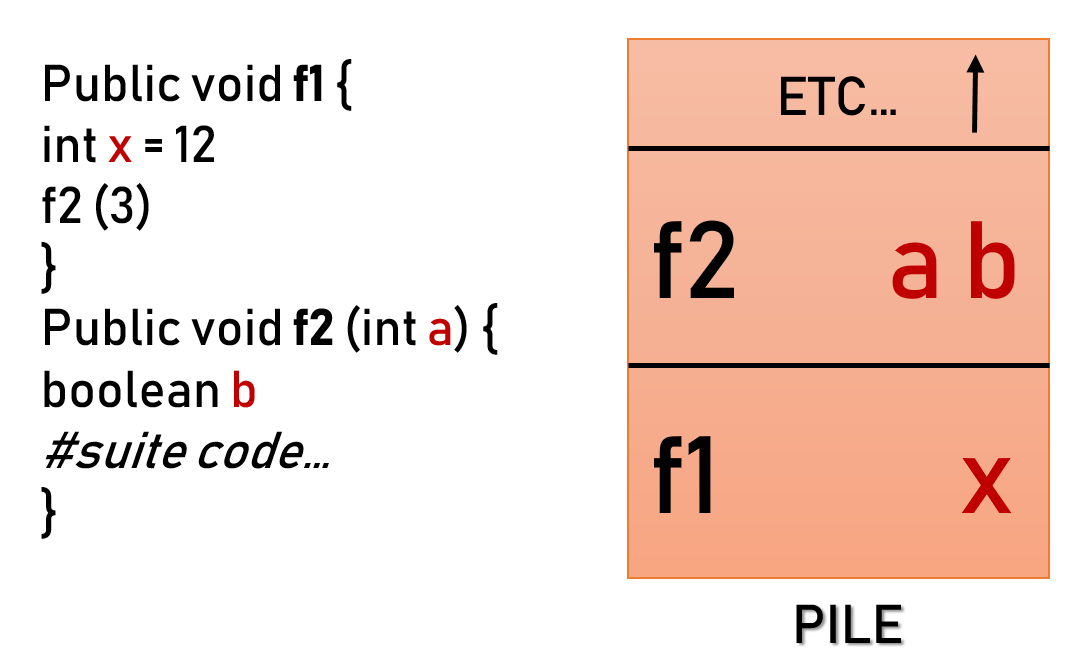
\includegraphics[width=0.5\linewidth,center]{pile_execution.png}\\
\\
\underline{Tas/Heap} : \\
\\
Le tas lui correspond au second segment de mémoire utilisé pour l’allocation dynamique. A la différence de la pile, vous êtes responsable de l’allocation de la mémoire sur le tas, avec l’utilisation de malloc() ou calloc() (fonctions C intégrées). Évidemment, vous devez également gérer l’utilisation de free () pour libérer cette mémoire dès que vous n’en avez plus besoin. Il est très important de le faire afin d’éviter les fuites de mémoire, qui provoquent la saturation de la mémoire machine.\\
\\
Les variables créées sur le tas sont accessibles par n’importe quelle fonction et n’importe où dans le programme, rendant leur portée globale. Il n’en fallait pas plus pour ajouter une contrainte supplémentaire : la gestion de l’accès concurrentiel (Quand 2 utilisateur veulent acceder a une meme ressource en meme temps).\\
\\
\underline{Pile ou Tas} : \\
\\
La mémoire sur le tas est plus grande et plus durable que sur la pile qui elle requiert une gestion plus complexe et donc plus lente .Le tas offre une bien plus grande liberté : au-delà de la portée globale des variables, celles-ci peuvent être redimensionnées à l’aide de la fonction realloc() ,la taille des variables dans le tas n’est pas limitée, du moins seulement par la limite physique de la mémoire.\\
\\
On peux montrer le schema suivant pour resumer cette partie sur la gestion de la memoire :\\
\\
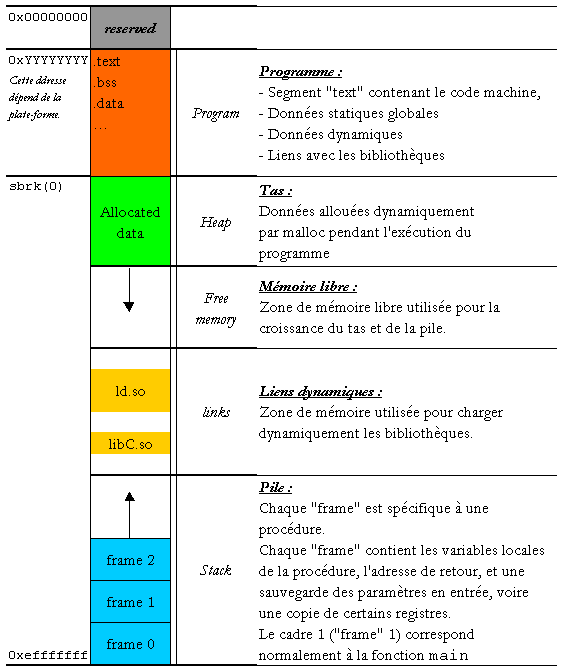
\includegraphics[width=0.5\linewidth,center]{gestion_memoire.png}\\
\\










\section{Arithmetique des pointeurs (Tableaux)}
\\
Il faut savoir que l'on peux addition , multiplier , soustraire et diviser des pointeurs entre eux mais cela ne presente pas beaucoup d'interet par contre on peut plutot le faire mais avec une constante et un pointeur .\\
Cela est utile pour parcourire et manipuler un tableau par exemple .\\
\\
\underline{Exemple} : \\
\begin{verbatim}
int i;
int T[N];
for(i=0;*(T+i)<N;i++){
  printf("%d\n",*(T+i));
}
\end{verbatim}
\\
Que fait ce bout de code , *(T+i) represente le debut du tableau point\'e T a l'adresse i si i=0 alors on commence au debut du tableau a l'adresse 0 , $T[i]=*(T+i)$.\\
En realite cela ce fait automatiquement par le compilateur , il traduite *(T+i) par :
\\
Pour i=0 , $(T+i)=(@T+i*$taille\_objet\_pointe$)=(T+0*4)=(T+0)$ debut du tableau , ceci est l'adresse si on veut le contenue $*(T+i)$ \\
taille\_objet\_pointe = 4 car c'est la taille du type int tout simplement.\\
Pour i=1 , $(T+i)=(T+1)=(T+1*4)=(T+4)$ 2ieme element du tableau \\
...\\
Pour i=N , $(T+i)=(T+N)=(T+N*4)=(T+N)$ Nieme element du tableau \\
\\
On se deplace de la taille de l'objet a chaque fois pour se deplacer dans le tableau .


\subsection{Tableau heterogene}
Pour ce deplacer dans un tableau heterogene , il suffit de se deplacer de la taille de l'objet .\\
Pour connaitre l'adresse de debut du tableau , peut importe le type ca sers toujour en (T+0) , mais si on veux aller sur le debut de la case du INT alors on se deplace de sizeof(char) pour arriver au debut de la case du INT.\\
\\
L'odrinateur calcule automatiquement les indice de la facons suivant : (T+i*Taille\_objet\_pointee) .\\
\\
\underline{Exemple} : \\
\\
\begin{verbatim}
char *T=malloc(sizeof(char));
printf("%c\n",*(T)); \\lecture 1er element
T=T+1; \\char = 1
printf("%d\n",*(int *)T); \\lecture 2ieme element
T=T+sizeof(int);
printf("%d\n",*(double*)T); \\lecture 3ieme element
T=T+sizoef(double) \\ deplacement a l'element suivant
...
\end{verbatim}










\section{Pointeur de Fonction}

-\underline{Declaration} e: \\
\\
\emph{type\_t  (\∗ptfonction ) (\ldots parametres \ldots);}\\
\\
-\underline{Exemple}:\\
\\
double(\∗F2 )(void)  ;        /\*Sans parametre\*/\\
int(\∗F3 )(int, S\_t \∗)  ;    /\*avec 2 parametres\*/\\
\\
Pour creer un affichage (ou autre) générique on peux déclarer des pointeurs de fonction dans la structure de l'objet :\\
\\
\begin{verbatim}
typedef struct entier_s entier_t ;

struct entier_s
{
  /* Attributs */
  int i ; 
  /* Methodes */  
  void (*afficher)(entier_t *) ;
  void (*incrementer)(entier_t *) ;
  void (*decrementer)(entier_t *) ;
} ;
\end{verbatim}
\\
Ou alors on peux creer une enumeration et faire une fonction d'aiguillage : \\
\begin{verbatim}
typedef enum message_s { AFFICHER , INCREMENTER , DECREMENTER } message_t ;

typedef struct objet_s objet_t ;

struct objet_s
{
  /* Attributs (vide) */
  /* Methodes (1 seule : aiguillage) */
  void (*switching)(objet_t * , message_t) ;
} ;

static
void afficher_int( entier_t * entier ) 
{
  printf( "%d\n" , entier->i ) ; 
} 

static
void decrementer_int( entier_t * entier ) 
{
  entier->i-- ; 
} 

static
void incrementer_int( entier_t * entier ) 
{
  entier->i++ ; 
} 

/* Corps aiguillage specifique a entier_t */
static
void switching_int( objet_t * self , message_t message ) 
{
  switch(message)
    {
    case AFFICHER :
      ((entier_t *)self)->afficher((entier_t *)self) ;
      break ; 
   case INCREMENTER :
      ((entier_t *)self)->incrementer((entier_t *)self) ;
      break ; 
    case DECREMENTER :
      ((entier_t *)self)->decrementer((entier_t *)self) ;
      break ; 
    }
} 


\end{verbatim}









\section{Encapsulation / Pointeur generique}
Le type void* permet de pointé sur n'importe qu'elle type d'objet (int,char,struct\_t,...) .\\
\\
\underline{Exemple} : \\
\begin{verbatim}
  int entier=5;
  int *pent=&entier;
  void *pgen;

  pgen=pent; //ok
  pent=pgen; //ko deferencement 

\end{verbatim}
\\
Un pointeur generique void* ne peux pas etre deferencé c'est a dire etre a droite de l'affectation .\\
\\
\underline{Utilité} : \\
Le principe d'utiliser des pointeur generique est de permettre de rendre des fonction generique capable de prendre en parametre n'importe qu'elle type d'objet on appelle cela l'encapsulation/call back.\\
On utilise une fonction classique qui fait sont traitement sur des int par exemple "void afficher\_int(int *entier)" et ensuite on cree une 2ieme fonction qui vas venir encapsuler la premiere grace aux pointeur generique "void afficher\_int (void *obj)" ou l'on retournera la 1ere fonction .
Il faut que "int entier" soit de type pointeur lors du passsage en parametre de la fonction "int *entier" sinon on ne pourras pas referencer le void* .\\  
\\
\underline{Exemple} : \\
\begin{verbatim}
#include <stdio.h>
#include <stdlib.h>

#include "test.h"
#define N 10

void afficher_int (int *ent){
  printf("%d\n",*ent);
  printf("Entier (int) : %d \n",*ent);
}

//Fonction qui encapsule et qui retourne la fonction pour le bon type d'objet
void afficher_int_cb (void * ent){
  return (afficher_int(ent));
}

void afficher_char(char *car){
  printf("Caractere (char) : %s \n",car);
}

void afficher_char_cb(void *car){
  return (afficher_char(car));
}

void afficher_string(char *string){
  printf("Chaine de caractere (char *) : %s \n",string);
}

void afficher_string_cb(void *string){
  return (afficher_string(string));
}

//Fonction generique qui permet de choisir les fonction d'encapsulation pour l'objet 
void afficher (void * obj,int val){
  if(val == 0){
    afficher_int_cb(obj);
  }
  else if (val == 1){
    afficher_string_cb(obj);
  }
  else{
    afficher_char_cb(obj);
  }
}

int main (int argc , char *argv[]){

  int ent;
  char car;
  char *string=malloc(sizeof(char *));
  printf("Entrez entier : ");
  scanf("%d",&ent);

  printf("Entrez chaine de caractere : ");
  scanf("%s",string);

  printf("Entrez un caracter : ");
  scanf("%s",&car);

  printf("\n\n");

  afficher(&ent,0);
  afficher(string,1);
  afficher(&car,2);

  free(string);
  string=NULL;

  return 0;
}
\end{verbatim}


%%%%%%%%%%%%%%%%%%%%%%%%%%%%%%%%%%%%%%%%%%%%%%%%%% STRUCTURE %%%%%%%%%%%%%%%%%%%%%%%%%%%%%%%%%%%%%%%%%%%%%%%%

\chapter{Structure}

\section{Type Structure}: \\

\unerline{Declaration} : \\
\begin{verbatim}
#DEFINE MAX 20

typedef struct s_individu {
      char nom[MAX] ;
      char prenom[MAX] ;
      struct individu * pere ;
      struct individu * mere ;
} t_individu ; 
\end{verbatim}
\\
De plus cette structure est recusif c-a-d que dans ca declaration elle s'appelle elle meme (\*pere,\*mere).\\
Ducoup si on declare une variable :\\
\textbf{Avec} typedef : t\_individu Nom\_var;\\
\textbf{Sans} typedef : struct s\_individu Nom\_var;\\
\\

\subsection{Passage en parametre de fonction}

Si on declare une variable de type t\_individu ,on feras un passage par addrese a la fonction pour utilise notre structure sans perdre de donnee.\\
exemple :\\
\\
\begin{verbatim}
int indiv_creer(t_individu *Indiv){
  
}

void main(){
  t_individu Indiv;
  indiv_creer(&Indiv);
}
\end{verbatim}


\section{Enumeration et Union}

\underline{Enumeration} : \emph{enum nom\_enum { val1, val2,\ldots, valN };}\\
\\
\underline{Union} : Se declare et s'utilise comme une structure .Contrairement a une structure une union ne peux contenir qu'un seul de ces membres a la fois. \\
\\
\begin{verbatim}
typedef struct nombre_s{
    unsigned entier : 1;
    unsigned flottant : 1;
    union
    {
        int e;
        double f;
    } u;
}nombre;

static void affiche_nombre(struct nombre n)
{
    if (n.entier)
        printf("%d\n", n.u.e);
    else if (n.flottant)
        printf("%f\n", n.u.f);
}
\end{verbatim}





%%%%%%%%%%%%%%%%%%%%%%%%%%%%%%%%%%%%%%%%%%%%%%%%%%%%%%%%%%%%%%%%%%%%%%%%%%%%%%%%%%%%%%%%%%%%%%%%%%

\chapter{Liste/Pile/File}

\textbf{LIFO}: signifie « Last In First Out ». Traduction : « Le dernier élément qui a été ajouté est le premier à sortir ».\\
 \\
\textbf{FIFO}: signifie « First In First Out ». Traduction : « Le premier élément qui a été ajouté est le premier à sortir » \\
\\


\section{Liste}

Les piles et files sont des liste chainée mais avec des accés aux elements plus particulier .Une liste chainée peux acceder aux elements de ces voisin grace a des pointeurs.\\


\section{Pile}

Une pile (stack) ,de type LIFO , est une liste ou chaque element a acces a l'element suivant en gardant un ordre d'empilage et depilage , on ne peux pas depiler le dernier element sans depiler ceux au sommet de la pile.\\
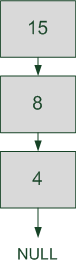
\includegraphics[height=0.35\textwidth,center]{pile_c.png}


\section{File}

Une file, de type FIFO , est une liste chainée ou chaque element a acces a l'element suivant en gardant les contraintes d'une liste ,on ne peux pas acceder directement au n-element de la liste sans la parcourire.\\
\\
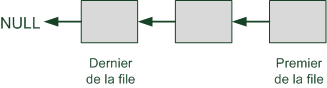
\includegraphics[width=0.5\textwidth,center]{file_c.png}

%%%%%%%%%%%%%%%%%%%%%%%%%%%%%%%%%%%%%%%%%%%%%%%%%%%%%%%%%%%%%%%%%%%%%%%%%%%%%%%%%%%%%%%%%%%%%%%%%%

\chapter{Trie}

Les algorithme de trie peuvent etre tres efficace comme tres lents , c'est pourquoi pour comparer 2 algorithme de trie on regarde leur complexite en O(n) , nombre d'instruction executer.\\



%%%%%%%%%%%%%%%%%%%%%%%%%%%%%%%%%%%%%%%%%%%%%%%%%%%%%%%%%%%%%%%%%%%%%%%%%%%%%%%%%%%%%%%%%%%%%%%%%%

\chapter{Recusitivité}

\section{Recusitivité}

\emph{Definition} : \\
Une fonction est dite recursive quand elle faut appele a elle meme pour traiter certaine operation .\\
Une fonction recursive doit avoir un "test d'arret" pour sortir de l'appel recursif .\\
\\
On creer autant de contexte d'execution qu'il y a d'appel de la fonction , il y a donc une place  memoire reserver pour les variable local de la fonction a chaque appel, c'est a dire que pour un  meme appele de fonction on auras differente variables local meme si elle portent le meme nom .\\
\\
\underline{Exemple} : \\
fact(n)--> sauvegarde de n en var local pour le 1er appel\\
fact(n)--> sauvegarde de n en var local pour le 2ieme appel\\
Pourtant les 2 n sont different ils portent le meme nom meme pas a la meme adresse .\\ 
\\
\textbf{Rappel} : Variable Global = 1 exemplaire $\neq$ Variable local = n exemplaire en memoire \\
\\
Un exemple de fonction recursive , la factoriel: \\
\begin{verbatim}
/* fonction qui renvoie n! */
int fact(int n) {
  if (n == 1)         //Condition d'arret
    return 1;
return n * fact(n-1); // Appel recursif
}

Appel : printf(‘‘%i’’, fact(3));
\end{verbatim}



\subsection{Recusitivite Terminal/Non-Terminal}
On dit qu'une fonction est Terminal quand la derniere instruction finit par l'appel de la fonction $\neq$ Non-Terminal .\\
\\
\underline{Exemple} : \\
\\
La fonction fact du dessus est non Terminal car la derniere instruction se finit par une multiplication (n*fact(n-1)) , le derniere terme est n et non fact() .\\
\\
Si on prend une version Terminal de la fonction fact cela donnerai : \\
\begin{verbatim}
/* fonction qui renvoie n! */
int fact2(int n, int result){
  if (n == 1)
    return result;
return fact2(n-1, n*result);
}

Appel : printf(‘‘%i’’, factorielle(3,1));
\end{verbatim}


\subsection{Derecursivation}


Toutes fonction recursive a une eccriture equivalente en \textbf{iterative} (en generale grace a une boucle while) on appele cela la \textbf{derecursivation} .\\
\\
On peux derecursiver une fonction non-terminal mais il faut prendre en compte la gestion d'une pile (stack) .

%%%%%%%%%%%%%%%%%%%%%%%%%%%%%%%%%%%%%%%%%%%%%%%%%%%%%%%%%%%%%%%%%%%%%%%%%%%%%%%%%%%%%%%%%%%%%%%%%%


\chapter{Arbre Binaire,ARN,N-aire}

Les arbres sont pratique pour la mise en place d'une structure de parcoure.\\

\section{Arbre Binaire}

\section{Arbre ARN}

\section{Arbre N-aire}







\end{document}
